\documentclass[letterpaper, 11 pt]{article}

\usepackage{amsmath}  % needed for \tfrac, \bmatrix, etc.
\usepackage{amsfonts} % needed for bold Greek, Fraktur, and blackboard bold
\usepackage{graphicx} % needed for figures
\usepackage{caption} 
\usepackage{hyperref}
\usepackage{float}
\usepackage{subcaption}
\setlength{\textwidth}{6.5in}
\setlength{\textheight}{8.5in}
\setlength{\oddsidemargin}{0pt}
\setlength{\evensidemargin}{0pt}
\setlength{\topmargin}{0pt}
\setlength{\marginparsep}{0pt}
\setlength{\marginparwidth}{1in}
\bibliographystyle{prsty}

% -------------------------------------------------------------------------------------
% BEGIN DOCUMENT
% -------------------------------------------------------------------------------------
\begin{document}
\title{Single Photon Experiments 2023}
\author{Tai Xiang}
\maketitle
\pagestyle{empty}

% -------------------------------------------------------------------------------------
% TABLE OF CONTENTS
% -------------------------------------------------------------------------------------
\tableofcontents
\newpage

% -------------------------------------------------------------------------------------
% INTRODUCTION
% -------------------------------------------------------------------------------------
All code and 3-D printing files can be found in the github resposity at \href{https://github.com/tyxiang0530/qrand}{https://github.com/tyxiang0530/qrand}.
\section{Single Photon Detection Set-up}

The basic set-up is based on the single photon lab developed at Dickinson college \cite{photon_setup}, involves a helium-neon laser in the IR band driven into a BBO crystal. Photons that enter the BBO crystal from the laser
undergo spontaneous parametric down-conversion and are then detected within two photon detectors, as shown in figure \ref{fig:spcm_setup_basic}.
\begin{figure}[H]
    \centering
    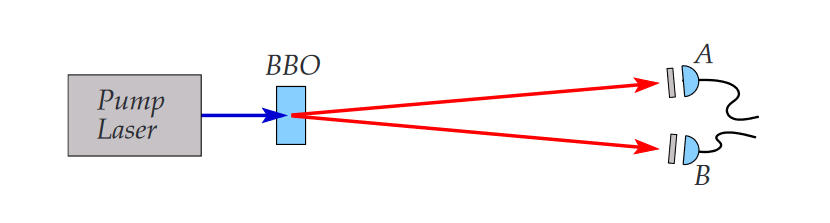
\includegraphics[width = 7cm]{setup_basic.png}
    \caption{Basic set-up for the SPCM experiment.}
    \label{fig:spcm_setup_basic}
\end{figure}

Additional beam-splitters can be added between the BBO and the detectors to
yield a set-up such as the one shown in figure \ref{fig:spcm_setup_bs}.
\begin{figure}[H]
    \centering
    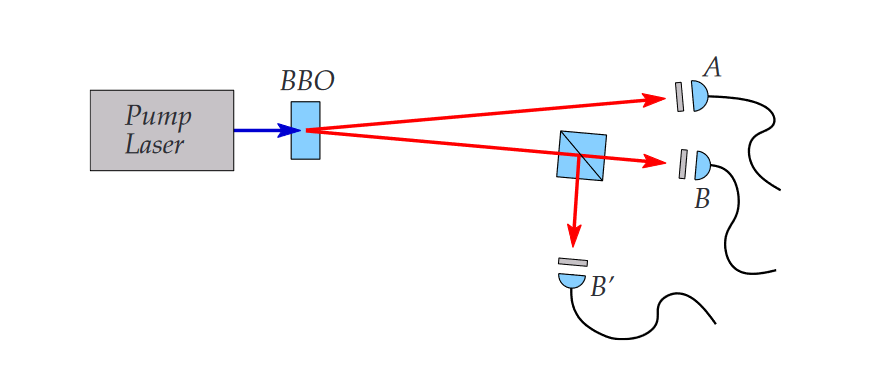
\includegraphics[width = 7cm]{setup.png}
    \caption{Beam-splitter set-up for the SPCM experiment.}
    \label{fig:spcm_setup_bs}
\end{figure}

This set-up will be the primary set-up used for the experiments and upgrades
listed in the later sections. 

Outputs from the detector set-up run to a single photon counter, the SPCM AQ4C.
To perform coincidence counting, they are sent to a coincidence counting module (CCM)
developed by Mark Beck \cite{beck_ccm}.

\section{Photon Statistics and Randomness}

One of the extensions I explored with the single photon counting module was to
apply it to the task of random number generation. Exploiting the quantum
intepretation of photons traveling within a beam-splitter and the Poissonian
nature of light, a high bitrate random number generator can be developed from
the current CCM experimental set-up. The random numbers generated from this
set-up can then be used to map out password strings or generate security keys.

With the beam-splitter source of randomness, the set-up generates random bits by
observing what detector measures a photon. In the set-up shown in figure
\ref{fig:spcm_setup_bs}, a 50--50 beam-splitter is placed between the detector B
and B'. In the quantum mechnical interpretation of light, the 50--50
beam-splitter causes an incident photon to have a 50--50 chance of arriving
within detector B or B'. Assigning a bit of 0 to B and a bit of 1 to B', we then
have a 50--50 chance of getting a bit of 1 or 0. By inserting an additional
detector A' that is analogous to B and B', and then adding a 50--50
beam-splitter between A and A', another random bit can be generated. 

Furthermore, since photons are emitted from the laser in a Poissonian nature, we
can split off a Poissonian distribution fitted to the count of arriving photons,
assign buckets to each, and draw random bits in accordance to what bucket a
time-step of photon counts falls into. This method is illustrated in figure
\ref{fig:poisson}.
\begin{figure}[H]
    \centering
    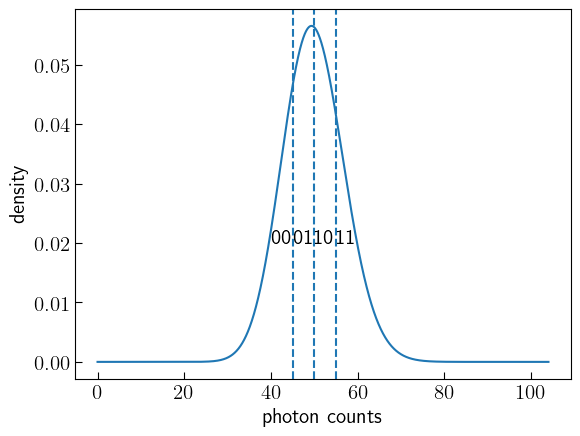
\includegraphics[width = 8cm]{poisson_cut.png}
    \caption{Poissonian distribution segmented into regions of equal area. A bit combination is then assigned to each region.}
    \label{fig:poisson}
\end{figure}

For example, taking an experiment fitted to the Poissonian displayed in figure
\ref{fig:poisson}, if there are 40 incident photons, then we get an output
bitstring of 01, if there are 45, we output 01, and so on. A Poissonian can be
drawn for each detector in the experiment. All software pertaining to the various
Poissonian operations mentioned in this report can be found in the python file PoissonianOps.py.

In an experiment with two beam-splitters and four detectors utilizing each of
the ports available on the SPCM-AQ4C module, a total bitrate of 10 bits per
integration time-step can be achieved. In the generation of a password or
security key, there are a total of 10 numbers, 40 symbols, 26 lower-case
letters, and 26 upper-case letters to choose from, yielding a total of 102
possible selections. A total of 7 bits can reach every outcome of
this, with $2^7 - 102 = 28$ additional mappings that are not used and can be
overflowed to the next time-step. Each experimental time-step generates 10 bits,
so we use 7 to generate a character and overflow the additional 3 bits as well
as the additional mappings to the next time-step for efficiency. 

We validate the random bits we generate with the NIST statistical test suite for
random number generates \cite{nist_sts}. The NIST statistical test suite contains a series of
tests utilized to determine the randomness of input number sequences \cite{sts_intro}. The
results of the tests are shown in table \ref{tab:rng_test}, where a score of
$8/10$ is considered passing.

\begin{table}[H]
    \centering
\begin{tabular}{|l|l|}
\hline
\textbf{Statistical Test}          & \textbf{Proportion} \\\hline
Frequency                 & 10/10      \\\hline
Block Frequency           & 10/10      \\\hline
Cumulative Sums           & 10/10      \\\hline
Longest Run               & 10/10      \\\hline
Longest Run (Rank)        & 10/10      \\\hline
Longest Run (FFT)         & 10/10      \\\hline
NonOverlapping Template   & 10/10      \\\hline
NonOverlapping Template   & 9/10       \\\hline
NonOverlapping Template   & 10/10      \\\hline
NonOverlapping Template   & 10/10      \\\hline
NonOverlapping Template   & 9/10       \\\hline
NonOverlapping Template   & 10/10      \\\hline
NonOverlapping Template   & 10/10      \\\hline
NonOverlapping Template   & 10/10      \\\hline
NonOverlapping Template   & 10/10      \\\hline
NonOverlapping Template   & 10/10      \\\hline
NonOverlapping Template   & 10/10      \\\hline
NonOverlapping Template   & 10/10      \\\hline
NonOverlapping Template   & 10/10      \\\hline
NonOverlapping Template   & 8/10      \\\hline
NonOverlapping Template   & 10/10      \\\hline
NonOverlapping Template   & 10/10      \\\hline
NonOverlapping Template   & 9/10      \\\hline
NonOverlapping Template   & 9/10      \\\hline
NonOverlapping Template   & 10/10      \\\hline
NonOverlapping Template   & 10/10      \\\hline
NonOverlapping Template   & 9/10      \\\hline
NonOverlapping Template   & 10/10      \\\hline
NonOverlapping Template   & 10/10      \\\hline
NonOverlapping Template   & 10/10      \\\hline
NonOverlapping Template   & 10/10      \\\hline
NonOverlapping Template   & 10/10      \\\hline
NonOverlapping Template   & 10/10      \\\hline
NonOverlapping Template   & 10/10      \\\hline
NonOverlapping Template   & 10/10      \\\hline
NonOverlapping Template   & 10/10      \\\hline
NonOverlapping Template   & 10/10      \\\hline
Random Excursions Variant & 10/10      \\\hline
\end{tabular}
\end{table}
\label{tab:rng_test}

The random numbers generated with our set-up pass the NIST statistical tests.
However, although the set-up performs extremely well on these tasks, it should
be noted that the passing of statistical tests is not a mathematically rigorous
definition of "randomness". The set-up merely performs well on human-defined
metrics of randomness.

To ensure that our experimental set-up is running accordingly and that there is
no systematic error that is causing non-Poissonian measurements, I have developed a
python file Main.py that has a method gen\_report that automatically generates a report that fits a set of
Poissonians to each randomness source we are relying on and investigates the fit.
The report generated also enables the user to analyze the CDF of each channel, as well
as a set of basic statistics for the given experimental run such as the count rate and the
total counts over time.


\section{Scattering Reduction}
An additional improvement I have made to this experimental set-up is the
development of multiple schemes to reduce scattering from background noise
sources. This section will cover a set of optimizations and developments on this
front.

\subsection{Black Paper and Boxes}

A very basic optimization that I performed to reduce scattering was to place
long sheets of black paper along the general beam-path of the laser. This was
done to ensure scattered light from sources external to the experiment, such as
light from the laptop screen and light from the controls of the coincidence
counting module, do not interfere with the experiment and generate accidental
coincidences.

Additionally, I also added a box that fits the optical components that are along
the beam-path prior to the BBO crystal. I cut a small hole that enables the beam
to travel into the box and another small hole that enables the beam to exit. Any
scattering that arises from the components inside the box is thus contained
within it and does not leak out into the room and contaminate the photons
arriving at the detectors. 

The additional pieces of paper along the beam-path as well as the box enclosure
as shown in figure \ref{fig:paper_scatter}.
\begin{figure}[H]%
    \centering
    \begin{subfigure}{.4\textwidth}
    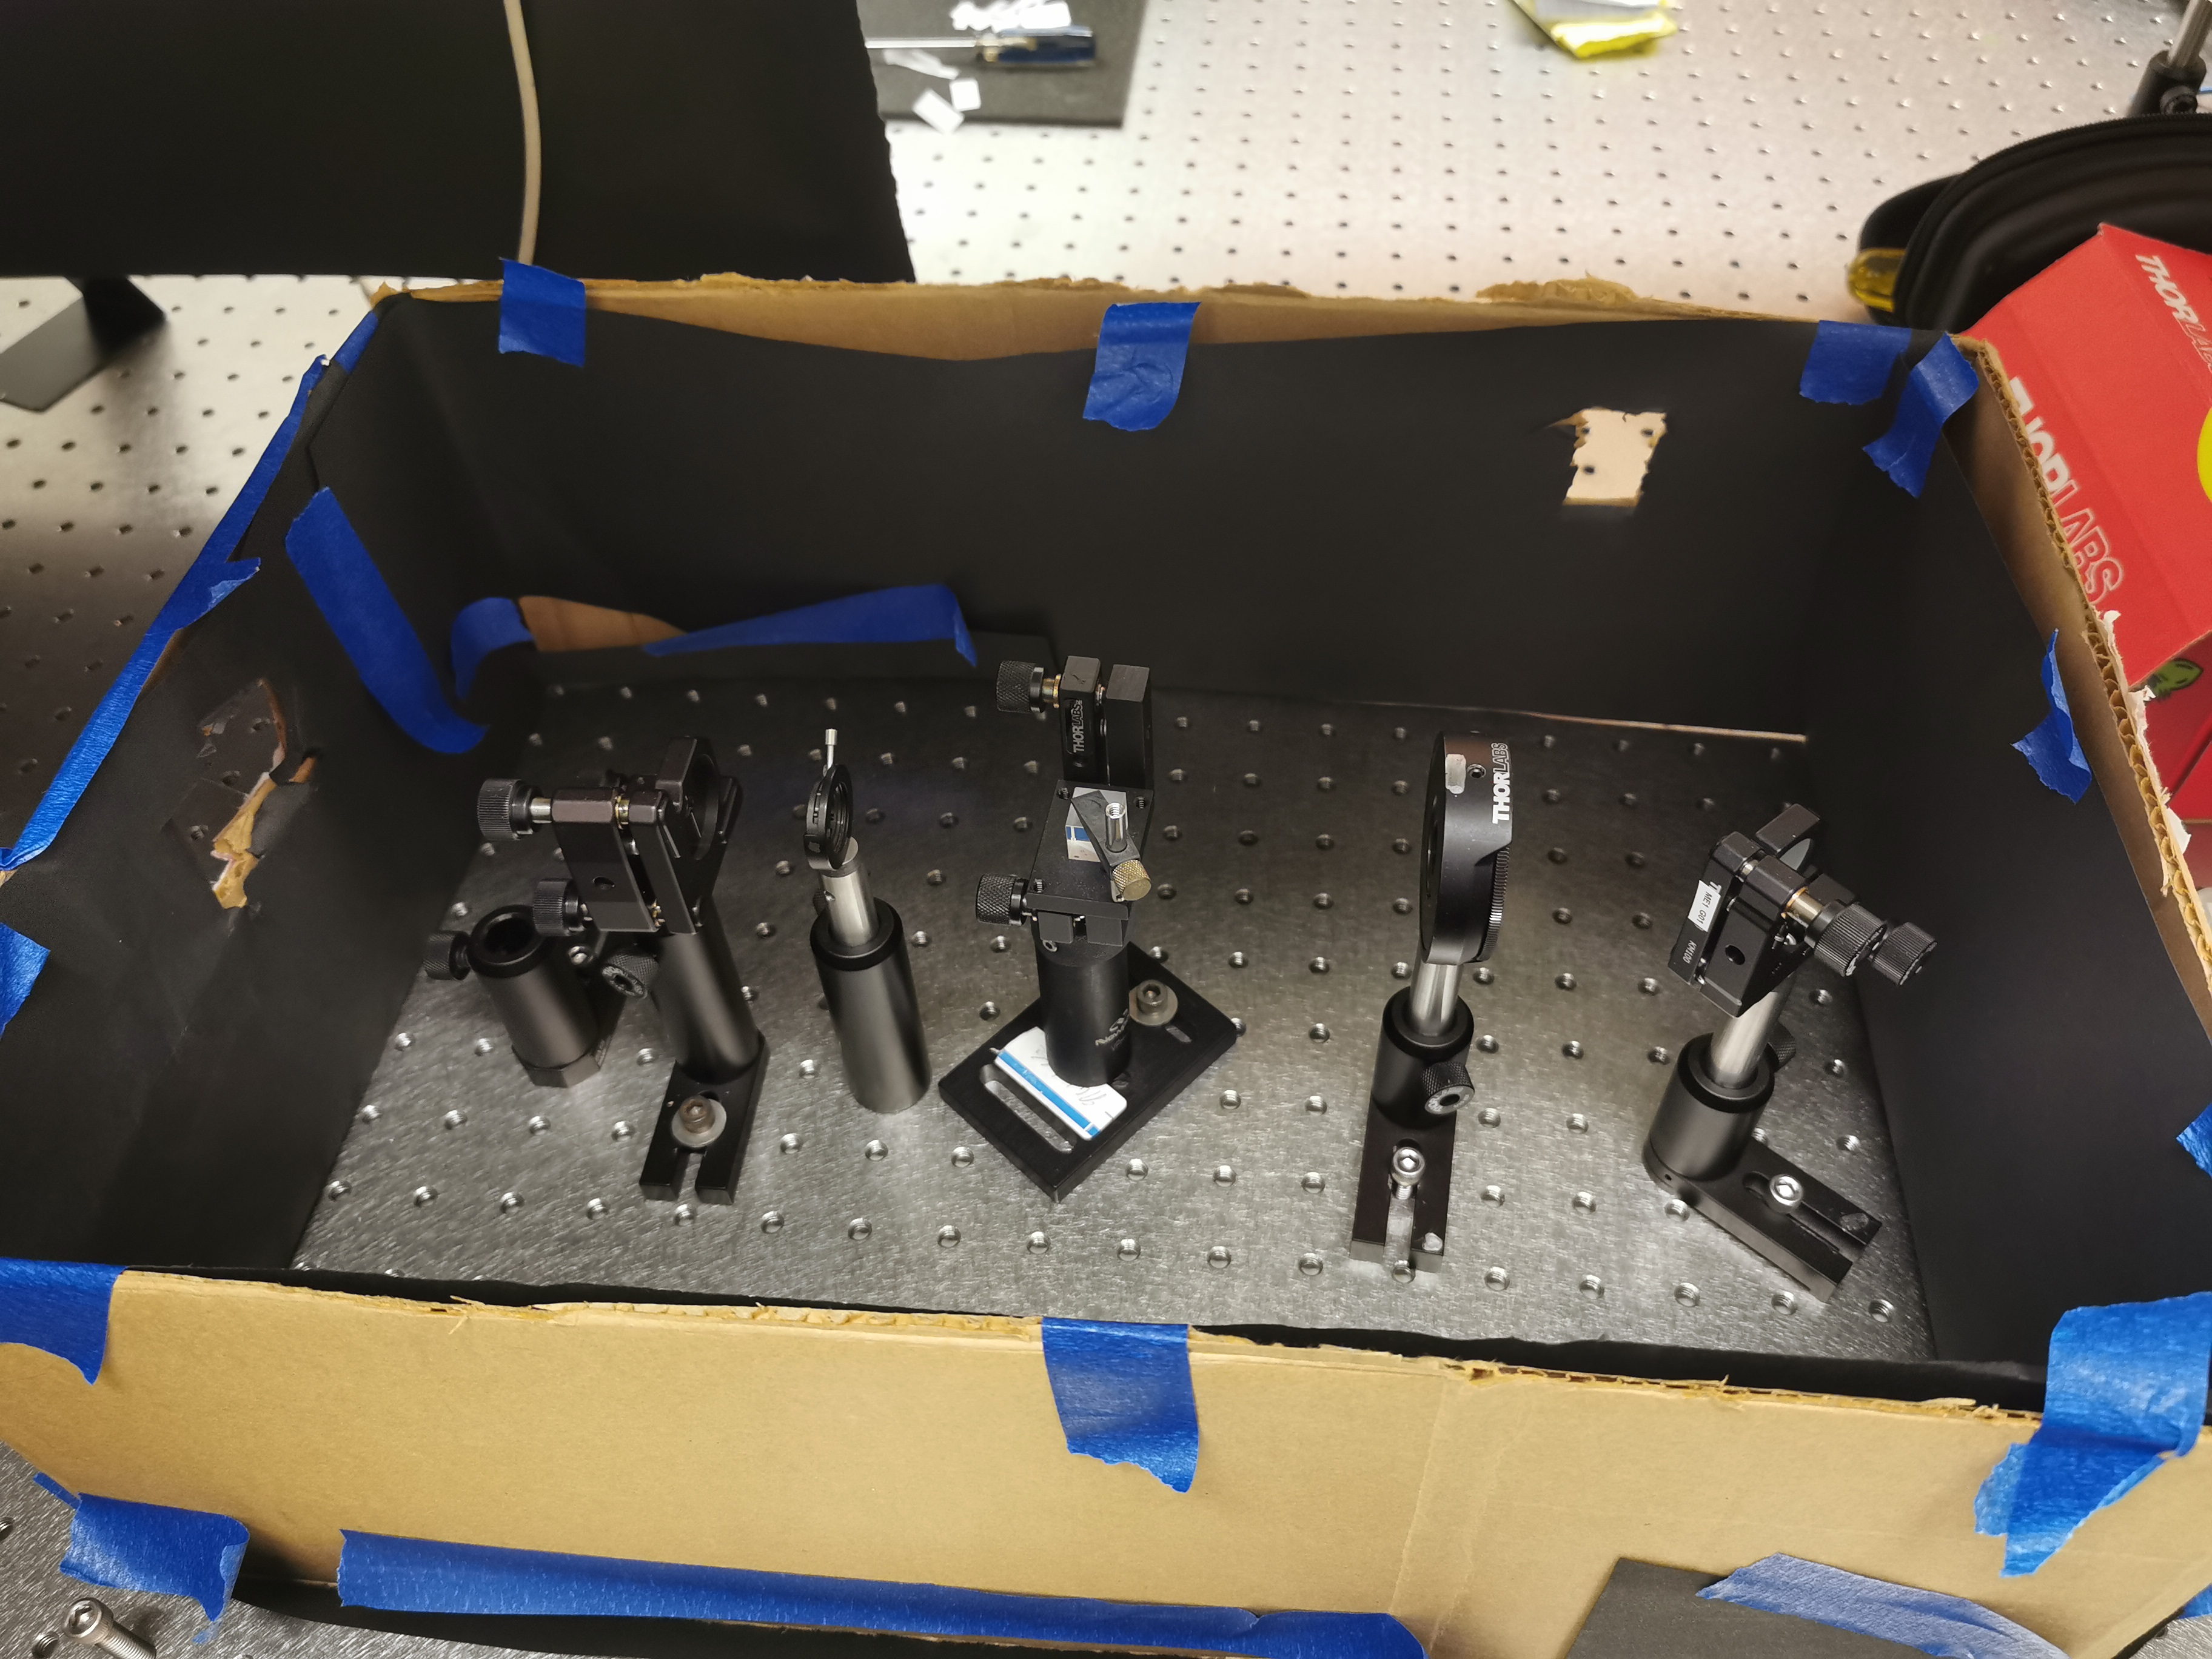
\includegraphics[width=7cm]{black_box.jpg}
    \caption{ }
    \label{fig:box}
    \end{subfigure}
    \begin{subfigure}{.4\textwidth}
    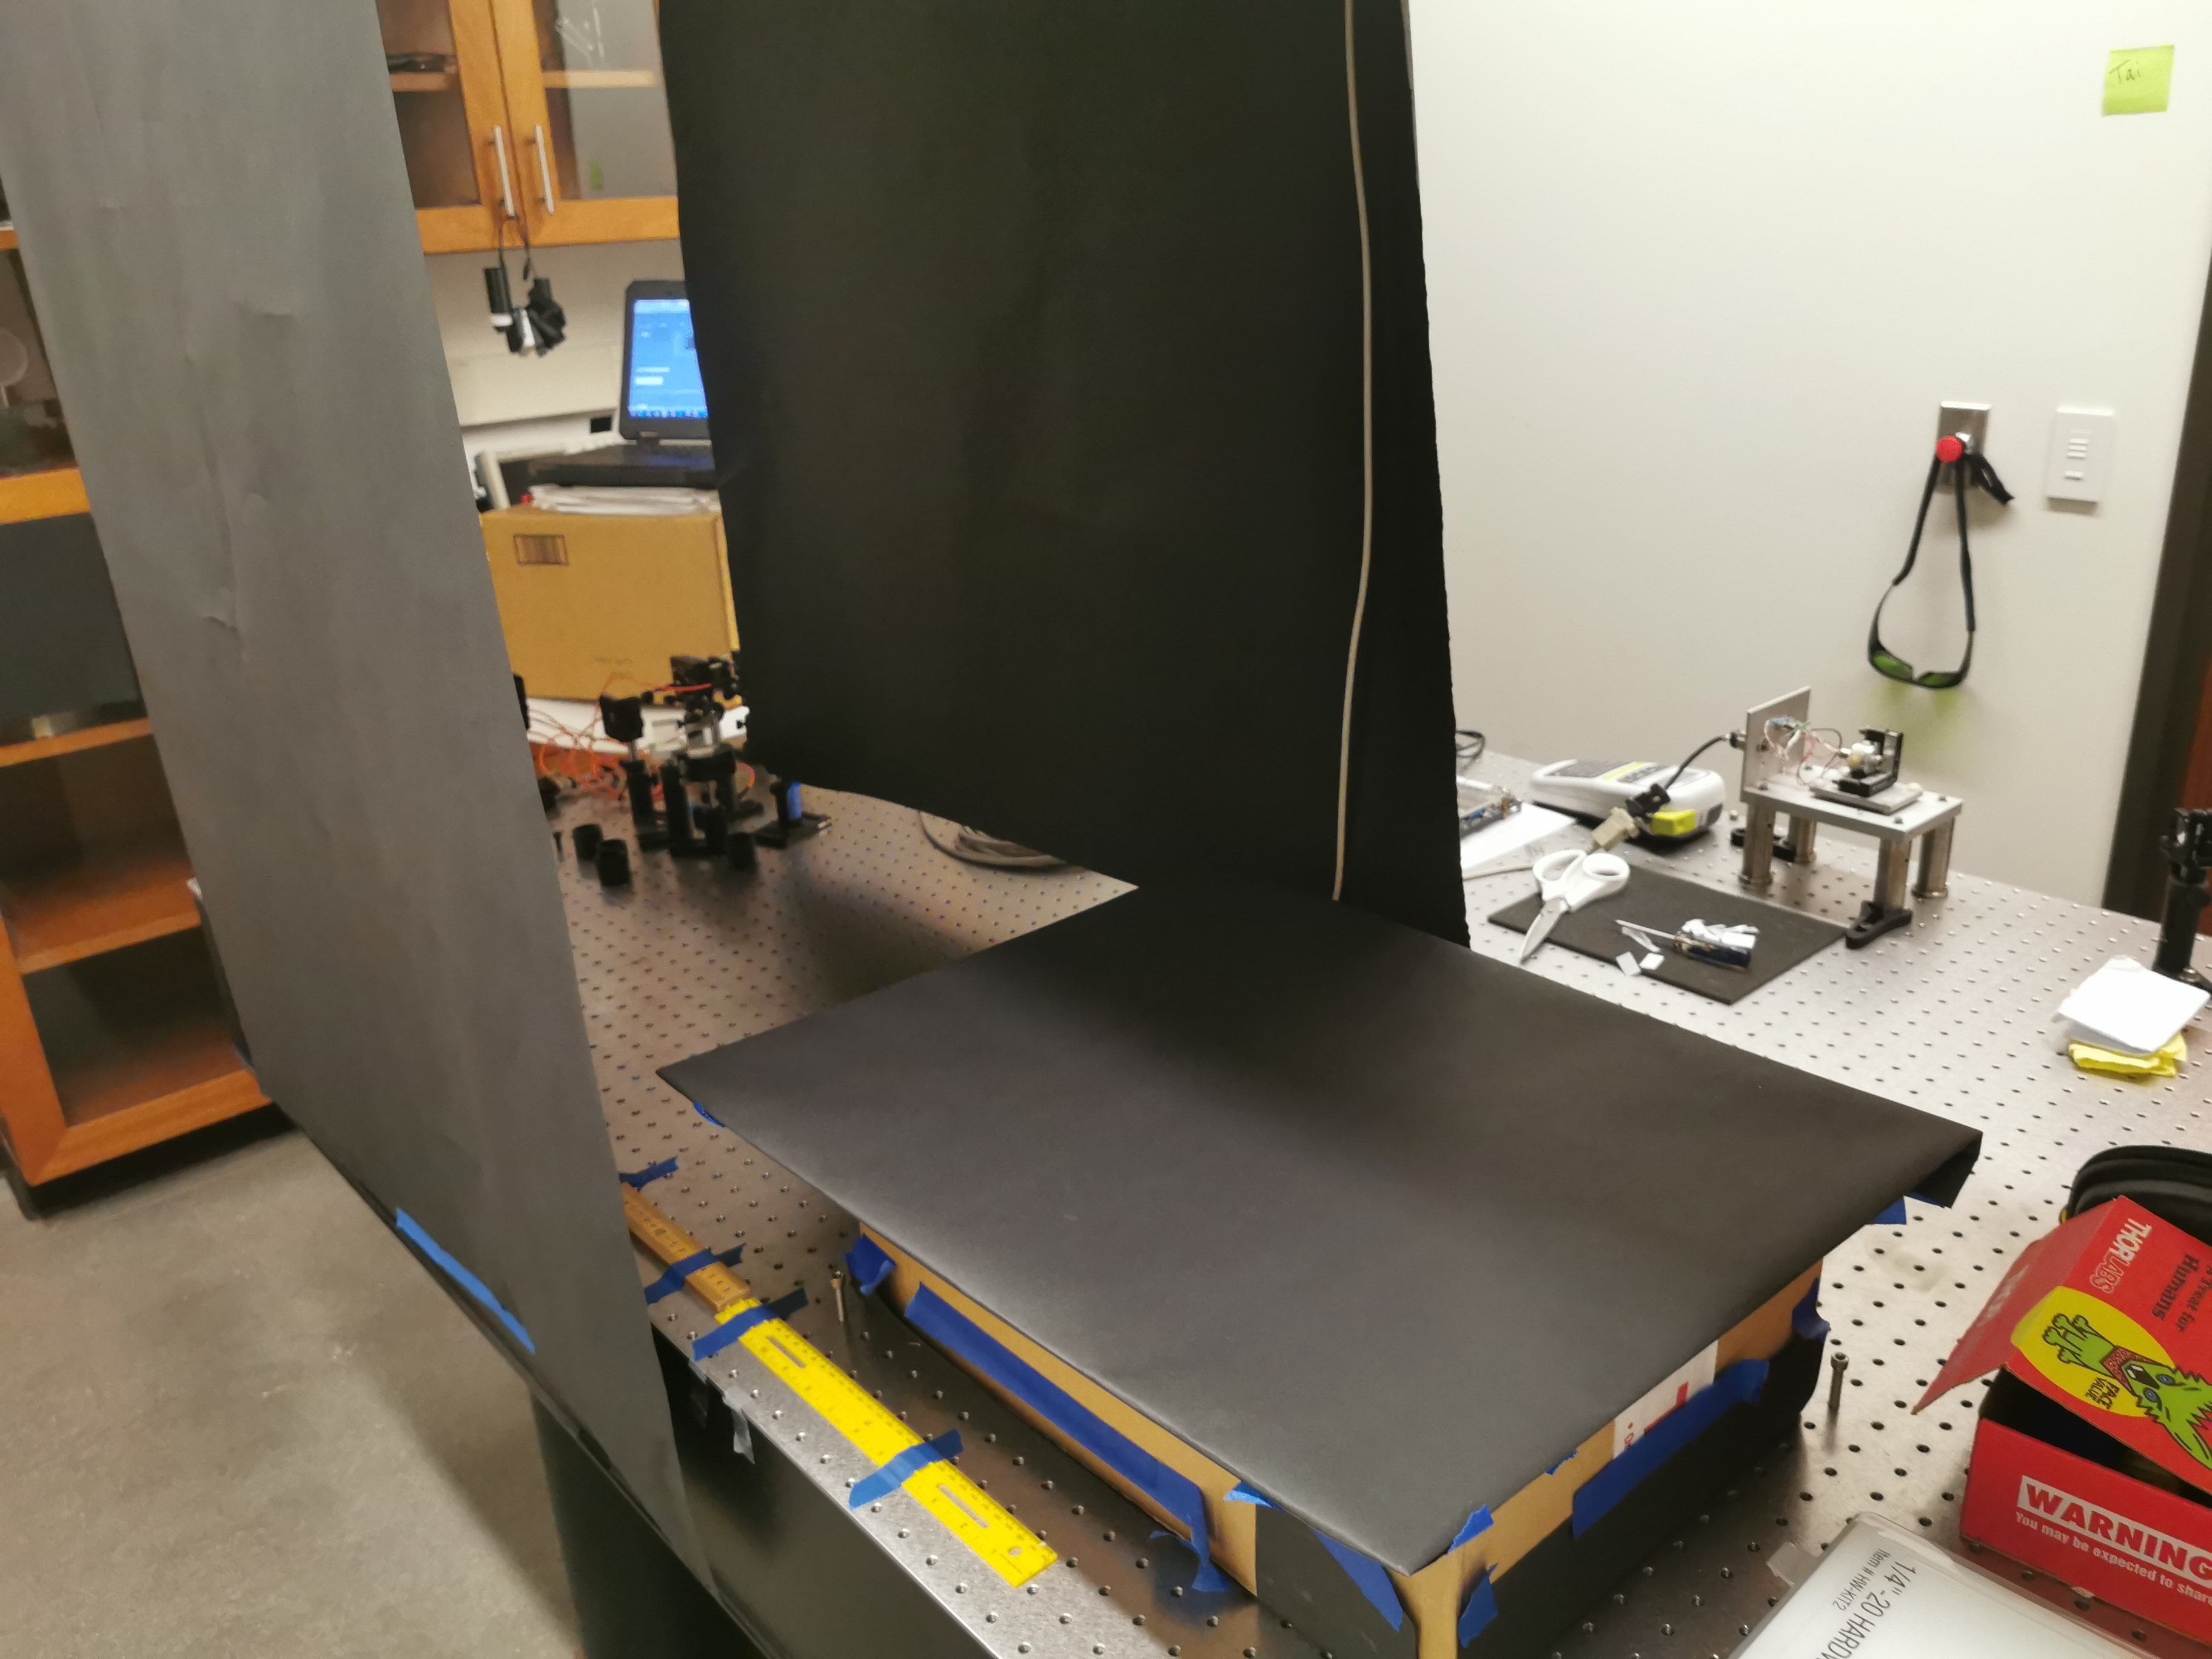
\includegraphics[width = 7cm]{black_surround.jpg}
    \caption{ }
    \label{fig:rail}
    \end{subfigure}
    \caption{Figure \ref{fig:box} shows the box that encloses the optical elements
    and figure \ref{fig:rail} shows the additional black paper placed around the experiment.}
    \label{fig:paper_scatter}
\end{figure}

\subsection{Enclosures}

Another scattering reduction optimization I have made is to create a 3-D
printable enclosure for the detectors that reduces the chance of entry for
noisey scattered photons. The two-piece enclosure fits and snaps over the
detectors and adds a cylindrical nose to the front. The long cylindrical nose
reduces the chance of photons that do not arise from the beam-path from hitting
the detector. The CAD designs are shown in figure \ref{fig:cad_enclose}.
\begin{figure}[H]%
        \centering
        \begin{subfigure}{.4\textwidth}
        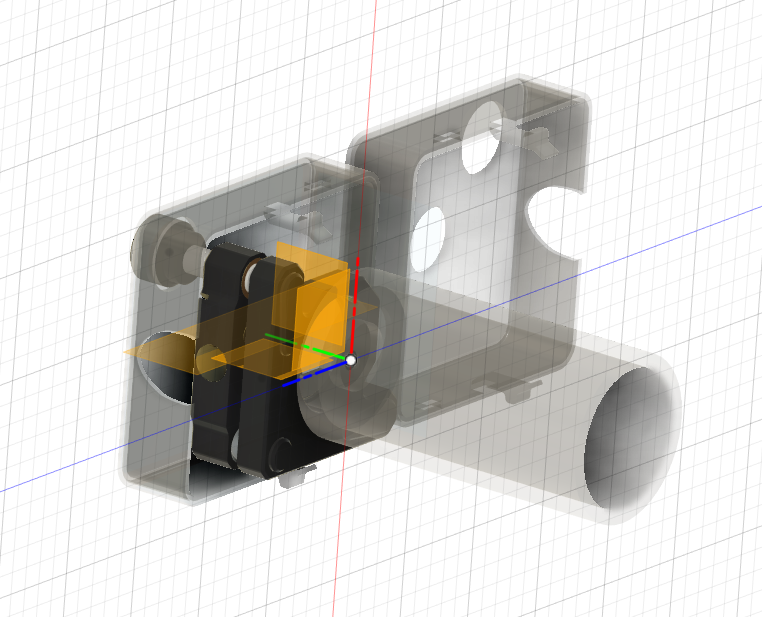
\includegraphics[width=7cm]{enclosure_1.png}
        \caption{ }
        \label{fig:side}
        \end{subfigure}
        \begin{subfigure}{.4\textwidth}
        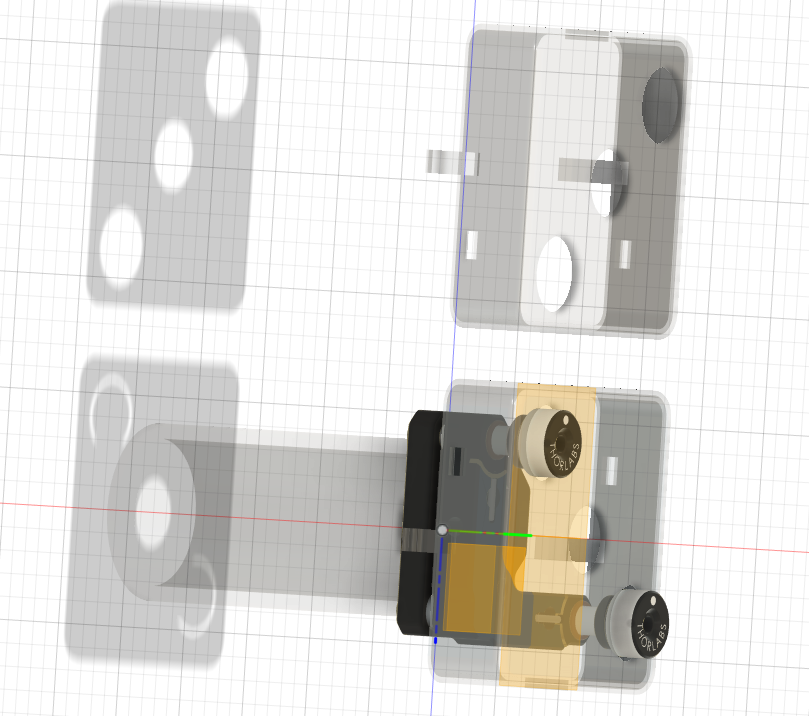
\includegraphics[width = 7cm]{enclosure_2.png}
        \caption{ }
        \label{fig:back}
        \end{subfigure}
        \caption{Figure \ref{fig:side} displays the side view of the enclosure.
        Figure \ref{fig:back} shows a back view. The two-piece enclosure snaps
        together through two joints and can easily be taken apart. The
        cylindrical nose must be glued on to the front of the enclosure.}
        \label{fig:cad_enclose}
    \end{figure}

Physically, the enclosure is shown in figure \ref{fig:phys_enclose}.
\begin{figure}[H]
    \centering
    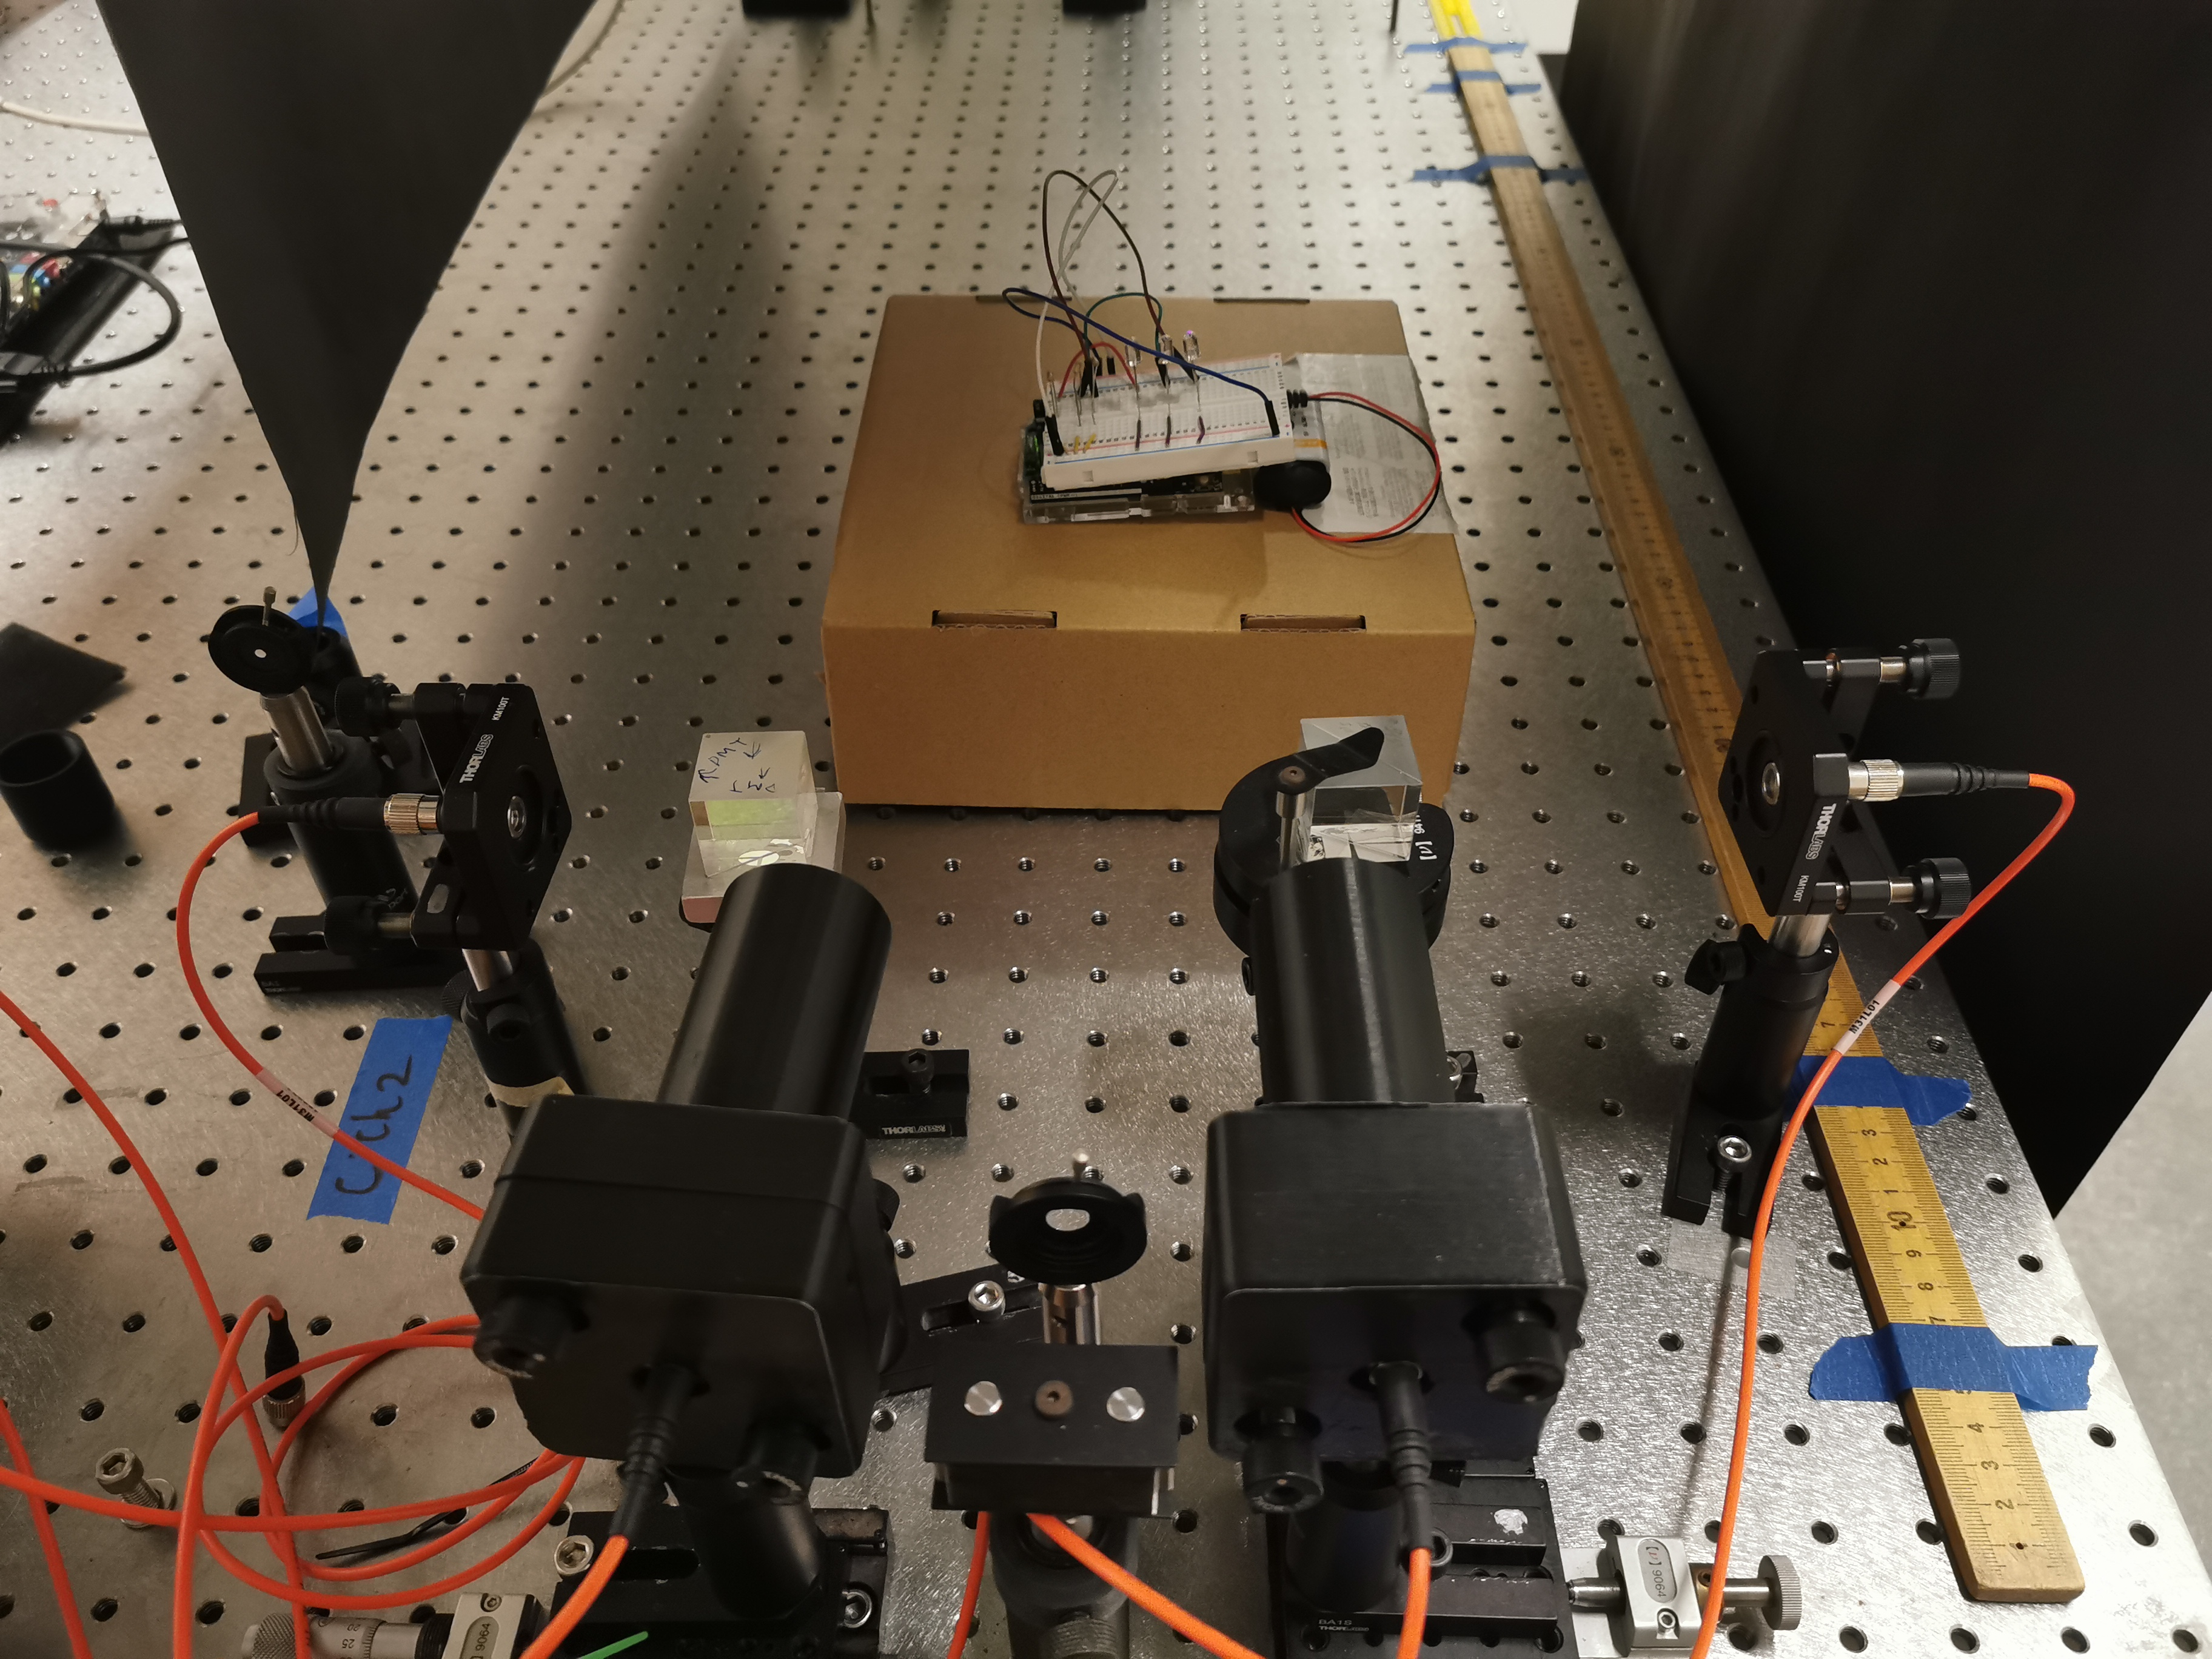
\includegraphics[width = 8cm]{enclose_phys.jpg}
    \caption{Enclosure inserted into experiment.}
    \label{fig:phys_enclose}
\end{figure}

The cylindrical nose-tube is also designed to fit a filter, such as the FR
RG780. When the enclosure was first designed, a different filter was used in the
experiment, and the experimental data we show later will be with the current filter, though a
later section will go on to discuss the use of the FR RG780. When these optimizations are applied to the basic experimental
set-up shown in figure \ref{fig:spcm_setup_basic}, we observe the results shown
in figure \ref{fig:scatter_reduce}.
\begin{figure}[H]%
    \centering
    \begin{subfigure}{.3\textwidth}
    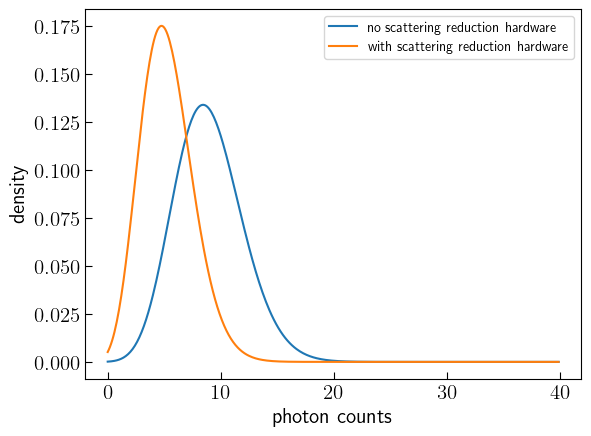
\includegraphics[width=5cm]{ch1_scatter.png}
    \caption{ }
    \label{fig:1}
    \end{subfigure}
    \begin{subfigure}{.3\textwidth}
    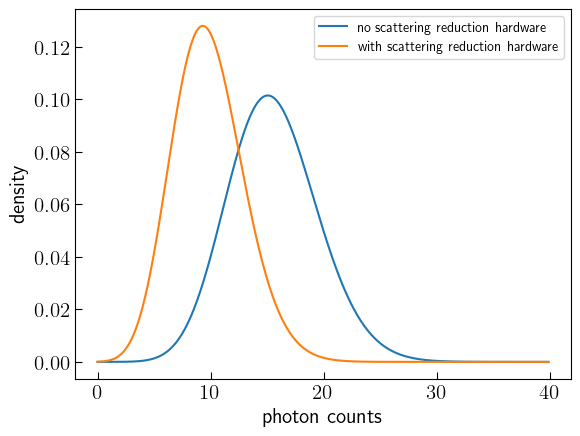
\includegraphics[width = 5cm]{ch2_scatter.png}
    \caption{ }
    \label{fig:2}
    \end{subfigure}
    \begin{subfigure}{.3\textwidth}
    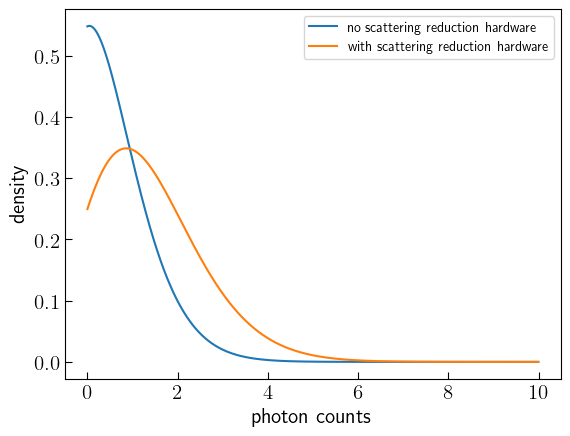
\includegraphics[width = 5cm]{cc_scatter.png}
    \caption{ }
    \label{fig:cc}
    \end{subfigure}
    \caption{Figure \ref{fig:1} shows the difference between the Poissonian
    distribution of photon counts per integration time-step in detector A with
    and without scattering reduction hardware. Figure \ref{fig:2} shows the
    difference between the Poissonian distribution of photon counts per
    integration time-step in detector B with and without scattering reduction
    hardware. Figure \ref{fig:cc} shows the difference between the Poissonian
    distribution of photon counts per integration time-step in A-B detector
    coincidences with and without scattering reduction hardware.}
    \label{fig:scatter_reduce}
\end{figure}

We observe that the scattering reduction steps that have been taken cut down on
the Poissonian mean of photon arrivals in channel A and B without a major
reduction in A--B coincidences. This suggests that the optimizations are cutting
out background nose but are not affecting the coincidences generated from
down-converted photons (the signal). 

\subsection{Filters}

Filters that only enable light in the IR range to pass through are effective in
reducing noise, as our laser operates in the IR range. At the beginning of the
experiment, we utilized a set of IR filters that were readily available in the lab. An easy optimization we can
make to the experiment is to improve the quality of the filter. We test the FR
RG780 in place of the current filters. The FR RG780 is a longpass filter with a filter
profile that is shown in figure \ref{fig:filter_prof}.
\begin{figure}[H]
    \centering
    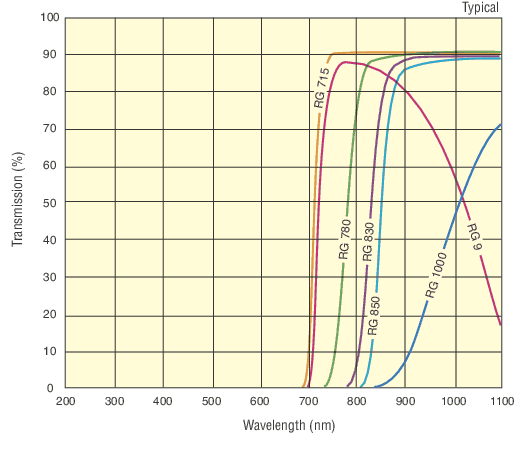
\includegraphics[width = 6cm]{COLOR_FILT_XMIT_8_600w.png}
    \caption{Filter profile of RG780 shown in green.}
    \label{fig:filter_prof}
\end{figure}

We compare the results of the experiment with no filter, with the current filters,
and with the new RG780 filters. We perform tests with the purple laser, a
maglite torch, and an IR LED array.

\subsection{Laser}
For the laser, when analyzing channel counts over time, we observe the results
shown in figure \ref{fig:filter_run}.
\begin{figure}[H]%
    \centering
    \begin{subfigure}{.4\textwidth}
    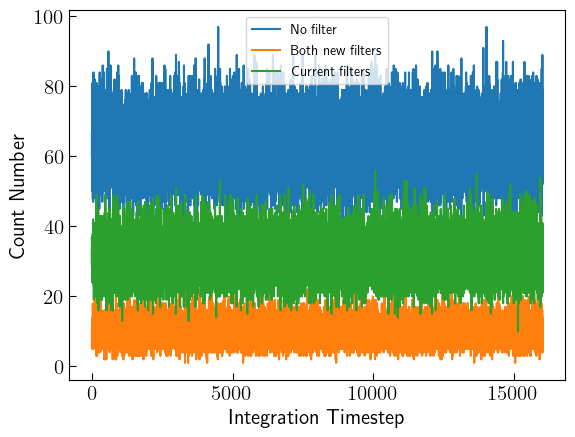
\includegraphics[width=6cm]{filter_ch1_laser.png}
    \caption{ }
    \label{fig:lch1}
    \end{subfigure}
    \begin{subfigure}{.4\textwidth}
    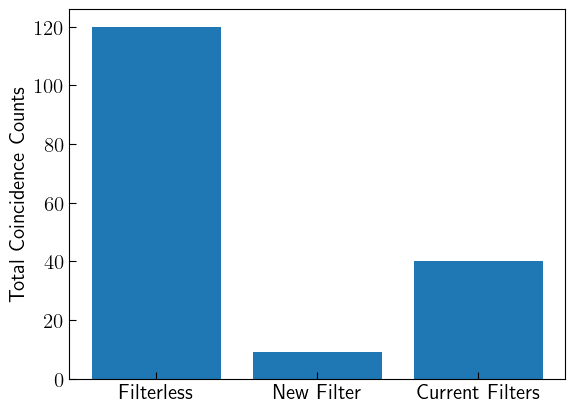
\includegraphics[width = 6cm]{filter_cc_laser.png}
    \caption{ }
    \label{fig:lcc}
    \end{subfigure}
    \caption{Figure \ref{fig:lch1} displays the count numbers measured over each
    integration timestep for a set-up with no filters, current filters in both the
    nose tube and following the output optical fiber, and the RG780 filter in
    both the nose tube and following the output optical fiber. Figure
    \ref{fig:lcc} shows the coincidences measured in each configuration.}
    \label{fig:filter_run}
\end{figure}
We observe that the variance in counts go down in accordance to 1 over the shot
noise, and we see that the RG780 filter outperforms the current filter in
regards to attenuation of the measured count numbers. The coincidence counts
also decrease. However, this is not enough to conclude that the RG780 filter is superior.

Another useful metric we can examine is the $\alpha$ value for each configuration.
$\alpha$ is the anticorrelation parameter. For two detectors and a channel for coincidence measurement,
we have
\begin{equation}
    \alpha_{2d} = \frac{R_c}{R^{(2r)}_{acc}}.
\end{equation}
Here, $R_{acc}$ denotes the rate of accidental coincidences and is defined to be
\begin{equation}
    R_{acc} = 2\tau R_1 R_2
\end{equation}
where $\tau$ is the coincidence window and $R_1$ and $R_2$ denote the count rates
for channel 1 and channel 2. $R_c$ denotes the coincidence rate. For correlated sources, 
such as photon pairs arriving from the single photon counting module (SPCM), we expect $\alpha > 1$.
For an uncorrelated source, such as white light from a torch, we expect $\alpha = 1$.

For each of the filter configurations, we can calculate some $\alpha$ value, finding the
results shown in table \ref{tab:alpha_laser}.
\begin{table}[H]
    \centering
    \begin{tabular}{|l|l|}
    \hline
    \textbf{Configuration} & \textbf{$\alpha$ Value} \\ \hline
    No Filters             & 0.645                   \\ \hline
    Current Filters        & 0.670                   \\ \hline
    RG780                  & 0.764                   \\ \hline
    \end{tabular}
    \caption{Table of $\alpha$ values for various filter configurations with a laser photon source.}
\end{table}\label{tab:alpha_laser}
Curiously, for the laser source, we do not observe an $\alpha$ that is greater than 1, which is
what we would expect for a correlated photon source. This defect will be addressed in section \ref{sec:ccm_broke}.
However, with the new RG780 filter, we achieve a higher $\alpha$ value, indicating that the accidental coincidences
from the experiment are decreases and we observe stronger correlation. This suggests that the RG780 filter outperforms
our current filters.

\subsection{Torch}
We perform the same set of tests described above with a maglite torch. The torch serves
as an uncorrelated photon source, and sends light outwards in a conal shape. We additionally test
this configuration to understand how well the new filter performs in the presence of a source
that primarily emits photons at a wavelength that is attenuated by the filter.

We once again examine the counts over time and the coincidences measured, though in this test
we omit the baseline filter-less case as the counts coming in are too high and excessively compress
the axis of our plots. We observe the results shown in figure \ref{fig:torch_filters}.
\begin{figure}[H]%
    \centering
    \begin{subfigure}{.4\textwidth}
    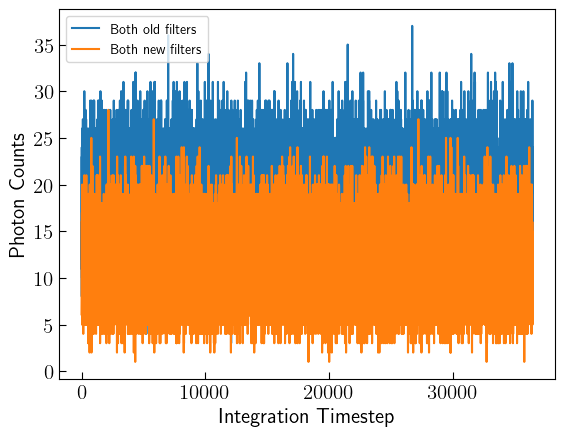
\includegraphics[width=6cm]{filter_ch1_torch.png}
    \caption{ }
    \label{fig:tch1}
    \end{subfigure}
    \begin{subfigure}{.4\textwidth}
    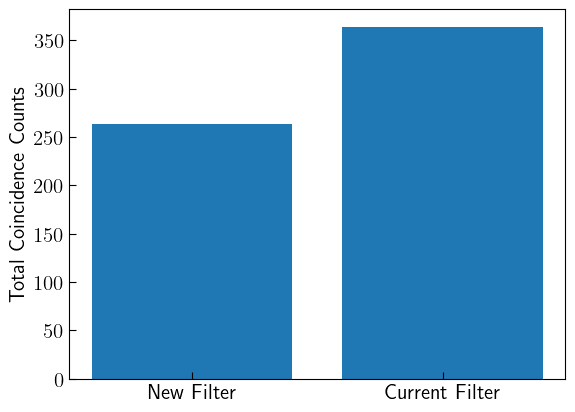
\includegraphics[width = 6cm]{filter_cc_torc.png}
    \caption{ }
    \label{fig:tcc}
    \end{subfigure}
    \caption{Figure \ref{fig:tch1} displays the count numbers measured over each
    integration timestep for a set-up with current filters in both the
    nose tube and following the output optical fiber and the RG780 filter in
    both the nose tube and following the output optical fiber. Figure
    \ref{fig:tcc} shows the coincidences measured in each configuration.}
    \label{fig:torch_filters}
\end{figure}
Once again, we witness an attenuation in counts and in coincidences. For the case of the
torch, we observe the $\alpha$ values shown in table \ref{tab:alpha_torch}.
\begin{table}[H]
    \centering
    \begin{tabular}{|l|l|}
    \hline
    \textbf{Configuration} & \textbf{$\alpha$ Value} \\ \hline
    Current Filters        & 0.638                   \\ \hline
    RG780                  & 0.677                   \\ \hline
    \end{tabular}
    \caption{Table of $\alpha$ values for various filter configurations with a torch photon source.}
\end{table}\label{tab:alpha_torch}
Interestingly, we once again observe results that contradict theory in that our $\alpha$ value
is not close to 1. However, we do once again observe that the RG780 filters outperform the current filters
in reducing the number of accidental coincidences and yielding a higher $\alpha$ value.

\subsection{IR LED Array}
We also examine the performance of our filters when an IR LED array is placed in front of
our detectors. This varies from the torch in that the wavelength of photons emitted by
the IR LED is in a range the filter does not attenuate. However, like the torch, the IR LED array source produces
uncorrelated photons and differs from the HeNe laser. We set-up our IR LED array in accordance with the schematic shown in figure \ref{fig:led_scheme}.
\begin{figure}[H]
    \centering
    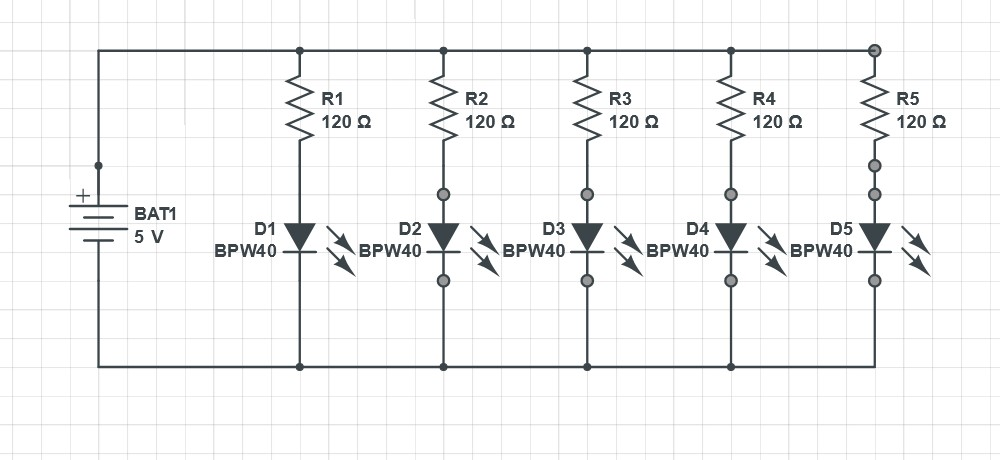
\includegraphics[width = 8cm]{IR_LED.jpg}
    \caption{Schematic of IR LED array}
    \label{fig:led_scheme}
\end{figure}
We perform the same measurements as those in the above sections and once again omit
the filterless detector due to high counts. We observe the results shown in figure \ref{fig:ir_comp}.
\begin{figure}[H]%
    \centering
    \begin{subfigure}{.4\textwidth}
    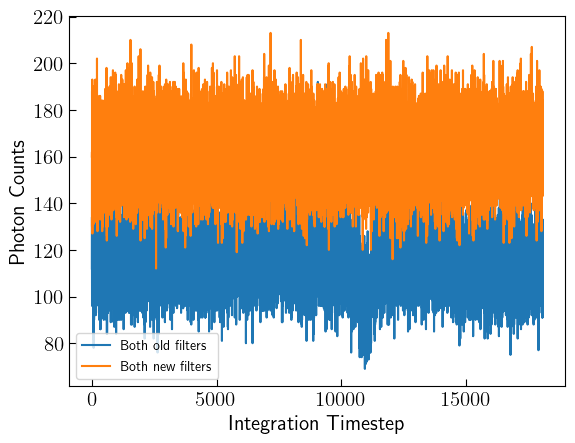
\includegraphics[width=6cm]{filter_ch1_IRled.png}
    \caption{ }
    \label{fig:irch1}
    \end{subfigure}
    \begin{subfigure}{.4\textwidth}
    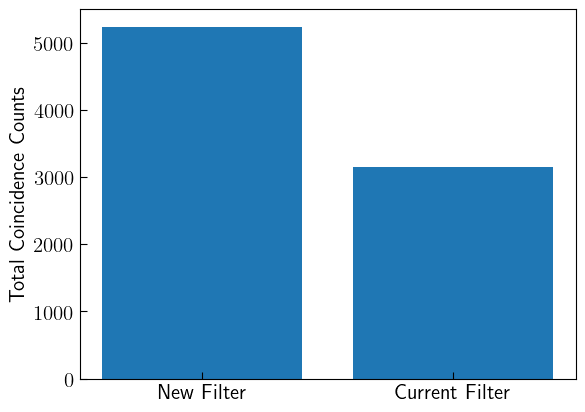
\includegraphics[width = 6cm]{filter_cc_irled.png}
    \caption{ }
    \label{fig:ircc}
    \end{subfigure}
    \caption{Figure \ref{fig:irch1} displays the count numbers measured with the IR LED array set-up over each
    integration timestep for a set-up with current filters in both the
    nose tube and following the output optical fiber and the RG780 filter in
    both the nose tube and following the output optical fiber. Figure
    \ref{fig:ircc} shows the coincidences measured in each configuration.}
    \label{fig:ir_comp}
\end{figure}

Interestingly, we observe that for the IR LED array, we observe a higher quantity of counts
with the RG780 than with the current filters. This suggests that the RG780 filter attenuates
the actual signal less, and has a steeper slope at the cutoff 780nm frequency. Ther current filter,
though it is at a similar band to that of the RG780, attenuates signal that it is not supposed to attenuate
at a higher rate, meaning it is likely an inferior filter and not as well made.

When we examine the $\alpha$ values for this set-up, we observe the values shown in
table \ref{tab:ir_cc}.
\begin{table}[H]
    \centering
    \begin{tabular}{|l|l|}
    \hline
    \textbf{Configuration} & \textbf{$\alpha$ Value} \\ \hline
    Current Filters        & 0.66                   \\ \hline
    RG780                  & 0.63                   \\ \hline
    \end{tabular}
    \caption{Table of $\alpha$ values for various filter configurations with a torch photon source.}
\end{table}\label{tab:ir_cc}

Here, we observe that the RG780 filter yields a lower $\alpha$ value than that of the 
current filter, suggesting that it measures more accidental coincidences than the
current filters. Though this is a negative, the strong cutoff and the high transmission of
photons within the signal bandwidth demonstrates that the RG780 is a superior filter than the current filter.

\section{Defects in Current Coincidence Counting Module (CCM)} \label{sec:ccm_broke}

In the previous section, we observe a set of measured $\alpha$ values that do not align with
theoretical results, namely the measurement of uncorrelated light yields $\alpha$s on the order of $10^{-1}$
and the measurement of correlated sources does not yield $\alpha > 1$.

We believe that this result is due to defects in the current coincidence counting module. To further
investigate this result, we analyze the pulse-shaper and the channel-by-channel variance of the counter
to better understand why this error may arise.

\subsection{Coincidence Windows and the Pulse Shaper}

We first analyze the pulse shaper in the CCM. The pulse shaper alters the waveform of a
photon detection event, decreasing the pulsewidths (equivalent to the parameter $\tau$) to those shown in table \ref{tab:pulsewidths}.
\begin{table}[H]
    \centering
    \begin{tabular}{|l|l|}
    \hline
    \textbf{Pulsewidth Setting} & \textbf{Pulsewidth} \\ \hline
    Short        & 10 $\pm$ 2.5ns                   \\ \hline
    Medium        & 14 $\pm$ 2.7ns                   \\ \hline
    Long        & 18 $\pm$ 2.8ns                   \\ \hline
    Unaltered                  & 25ns                   \\ \hline
    \end{tabular}
    \caption{Table of $\alpha$ values for various filter configurations with a torch photon source.}
\end{table}\label{tab:pulsewidths}
Coincidences are measured by examing waveform overlaps between two
detectors, and thus a decrease in pulsewidth may lead to a decrease in accidental coincidences,
as two waveforms must arrive within a smaller increment of time for overlap,
and subsequently coincidence to occur.

We investigate the $\alpha$ values yielded for different pulsewidths.
\begin{table}[H]
    \centering
    \begin{tabular}{|l|l|}
    \hline
    \textbf{Pulsewidth Setting} & \textbf{$\alpha$} \\ \hline
    Short        & 0.653                   \\ \hline
    Medium        & 0.755                   \\ \hline
    Long        & 0.748                   \\ \hline
    Unaltered                  & 0.930                   \\ \hline
    \end{tabular}
    \caption{Table of $\alpha$ values for various filter configurations with a torch photon source.}
\end{table}\label{tab:pulsewidths}
We find these results to be quite odd. A scaling of $\alpha$ with the pulsewidth can be expected,
as an increase in pulsewidth leads to an increase in coincidences, as pulses from the two detectors are now
more likely to overlap. However, the scaling at which this occurs, especially where medium and long equal one another, is rather strange and unexpected. This leads us to believe that there may something wrong with our pulse-shaping circuit.

We first validate the pulse-shaper settings by measuring output waveforms from the CCM on an oscilloscope.
The pulsewidths are sound, and align well with the values we have in table \ref{tab:pulsewidths}. We
next turn to investigating the channels of the CCM.

\subsection{Channel Variance}

We continue to investigate the current CCM and analyze if there is any variance when the detectors
are put into differing input channels. If some variance occurs, this would suggest that there is some
inconsistency between the various inputs of the CCM. We put detectors A and B into channel 1 and 2,
channel 2 and 3, and channel 3 and 4, with each taking measurements from the same experimental system.
We measure $\alpha$ for each, observing the results shown in table \ref{tab:alpha_channelvar}.
\begin{table}[H]
    \centering
    \begin{tabular}{|l|l|}
    \hline
    \textbf{Pulsewidth Setting} & \textbf{$\alpha$} \\ \hline
    1, 2 input        & 0.830                   \\ \hline
    2, 3 input        & 0.651                   \\ \hline
    3, 4 input        & 0.685                   \\ \hline
    \end{tabular}
    \caption{Table of $\alpha$ values for different channel inputs.}
\end{table}\label{tab:alpha_channelvar}
This drastic variance in $\alpha$ value suggests that there is something wrong with our CCM.
Each experimental run takes measurement from the same system, and the CCM ought to process inputs
from different channels in the same manner. However, we see that in the results shown in table \ref{tab:alpha_channelvar},
this is not the case.

\section{Altera DE-2 FPGA CCM}

Due to the age and myriad of issues that we have found in the current CCM,
we seek to develop an alternative coincidence counting unit with an Altera DE-2 FPGA CCM.
This is based upon the information provided from Mark Beck and their DE-2 coincidence unit.

The Altera DE-2 is a design and education board with a wide variety of uses. We primarily leverage it
for the Cyclone FPGA in the system and use it to count coincidences. Similar to the current CCM,
the Altera FPGA can take in a set of ttl signals, check for overlap between the signals, and count coincidences.
Like the current CCM, the Altera FPGA is easily programmable and has a high enough bit count to measure every possible
combination of coincidences for a four input experiment (A, A', B, B').

\subsection{Breakout Board}

To convert the output TTL signals from the SPCM AQ4C, we need a breakout board to convert
the output signals into 3.3V logic signals, which the Altera FPGA uses. To do this, we utilize
the schematic for our voltage divider shown in figure \ref{fig:divide}.
\begin{figure}[H]
    \centering
    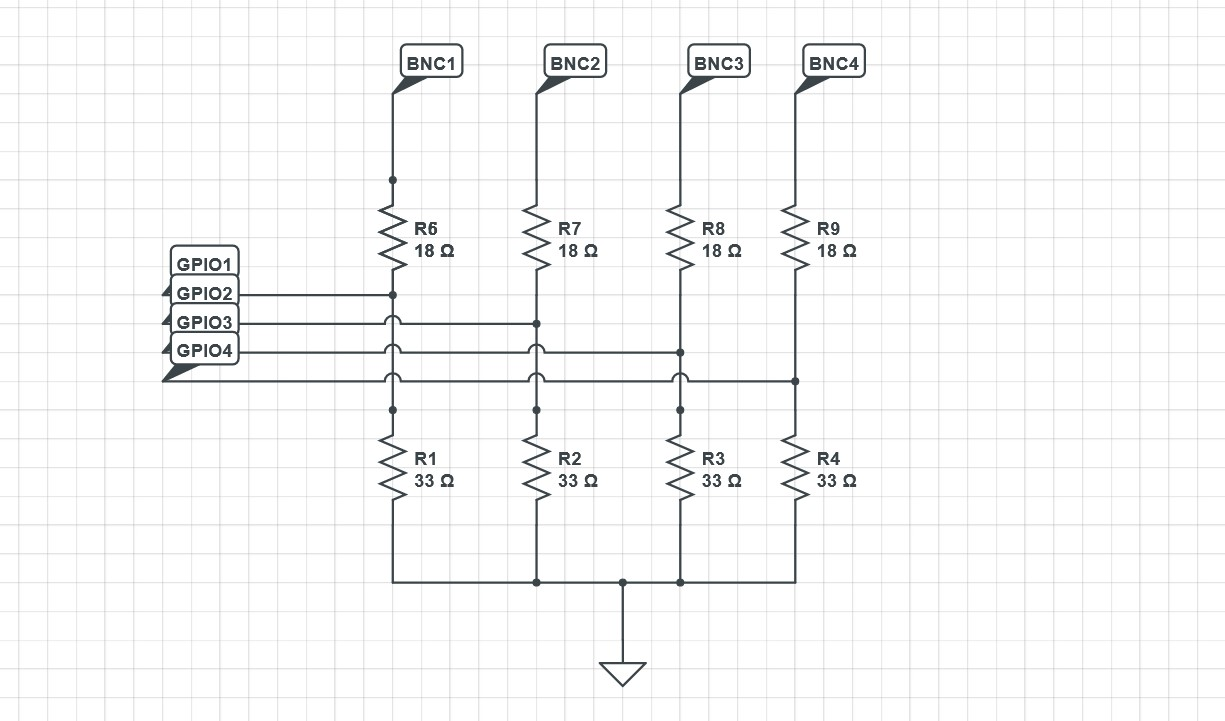
\includegraphics[width = 8cm]{BB_schematic.jpg}
    \caption{Breakout board schematic.}
    \label{fig:divide}
\end{figure}
Signals enter into the circuit through four individual BNC inputs for each channel and exit through a ribbon cable and then into the DE-2
GPIO inputs. The full breakout board is shown in figure \ref{fig:bb}.
\begin{figure}[H]%
    \centering
    \begin{subfigure}{.4\textwidth}
    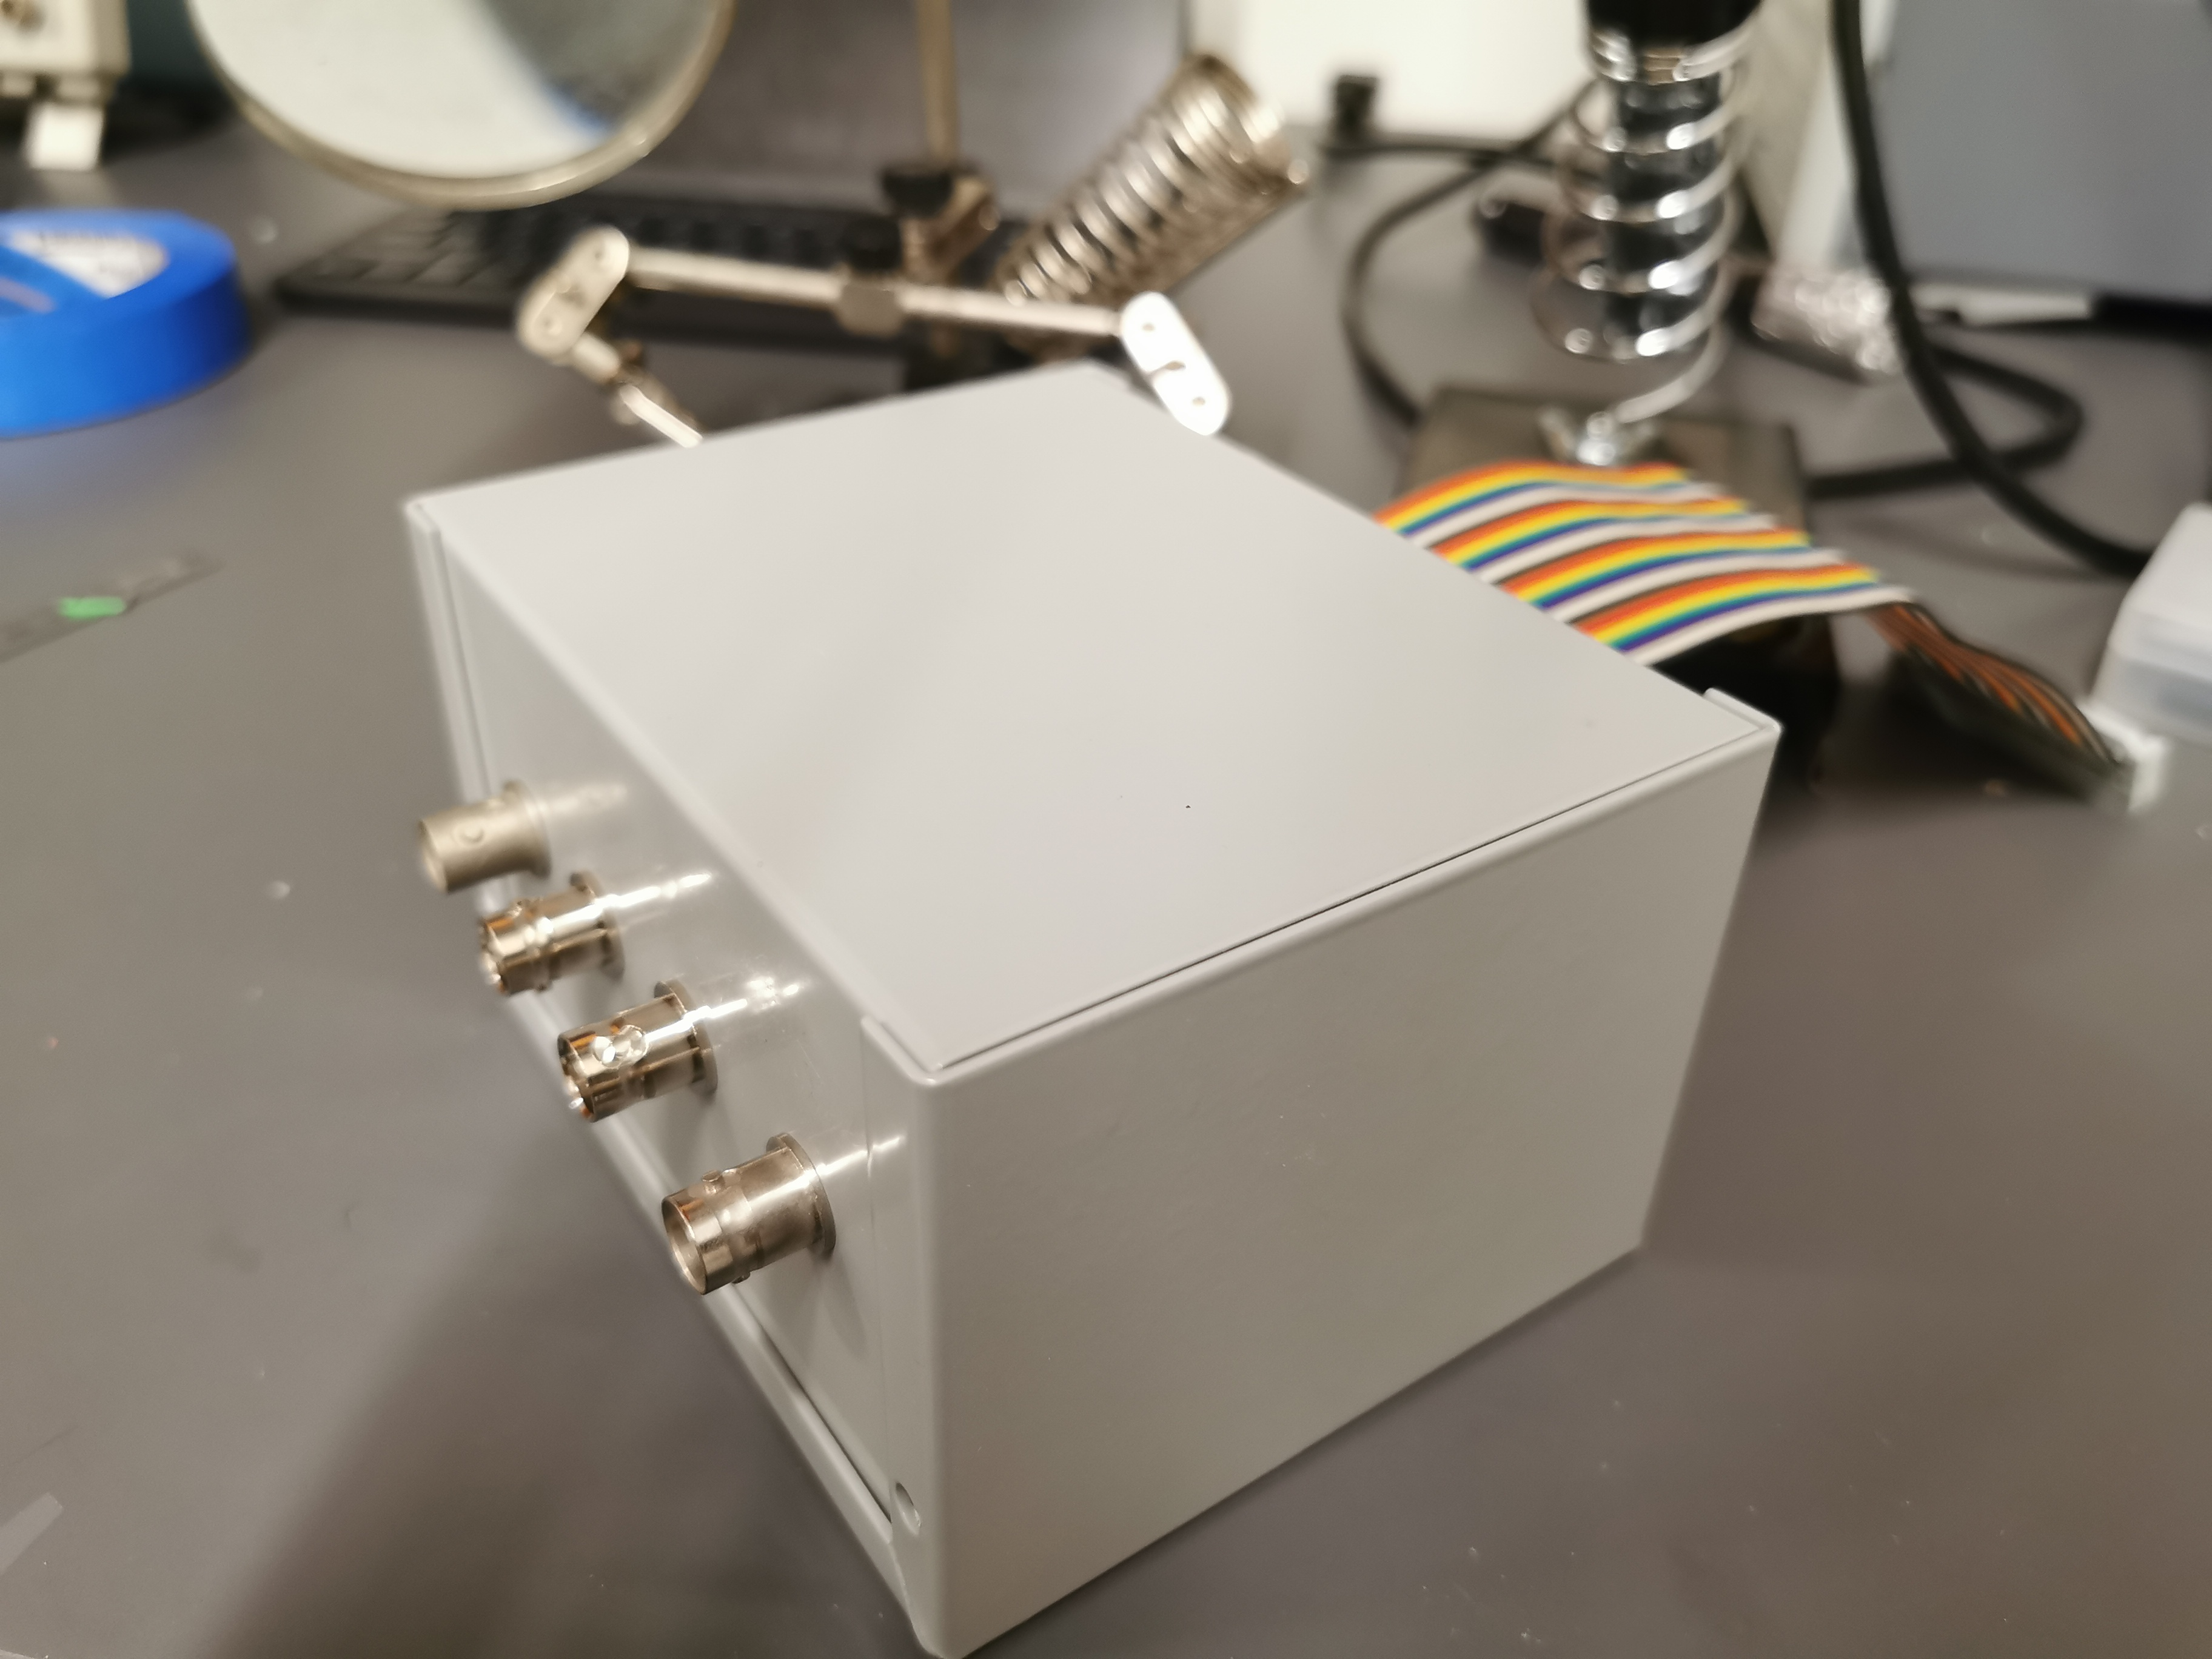
\includegraphics[width=6cm]{BB_box.jpg}
    \caption{ }
    \label{fig:box}
    \end{subfigure}
    \begin{subfigure}{.4\textwidth}
    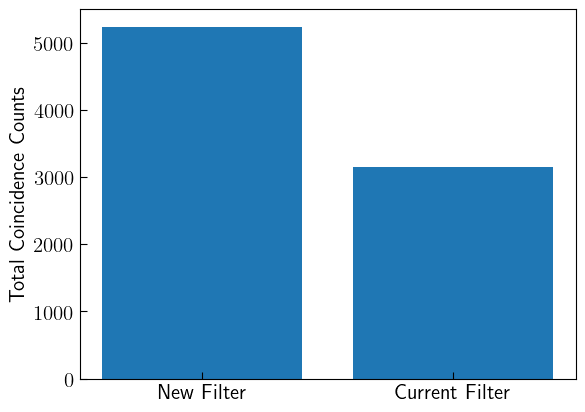
\includegraphics[width = 6cm]{filter_cc_irled.png}
    \caption{ }
    \label{fig:circ}
    \end{subfigure}
    \caption{Figure \ref{fig:box} displays the enclosure for the breakout board circuit.
    Figure \ref{fig:circ} displays the implemented breakout board circuit}
    \label{fig:bb}
\end{figure}

It should be noted that there are only 4 GPIO pins that are used on the FPGA, and thus outputs
from the voltage divider must be connected to the correct pins on the ribbon cable to ensure
that the four GPIO pins are correctly addressed. Here, we use
a raspberry pi ribbon cable, and thus each of the inputs must be sent to the raspberry pi ribbon cable
inputs in accordance to table \ref{tab:gpioin}.
\begin{table}[H]
    \centering
    \begin{tabular}{|l|l|l|}
    \hline
    \textbf{Channel} & \textbf{Pi Input} & \textbf{FPGA Input} \\ \hline
    1        & 1 &  GPIO13                 \\ \hline
    2        & 2 &    GPIO15              \\ \hline
    3      & 3 &        GPIO17         \\ \hline
    4      & 4 &          GPIO19       \\ \hline
    gnd      & 4 &          GPIO12       \\ \hline
    gnd     & 4 &          GPIO14       \\ \hline
    gnd      & 4 &          GPIO16       \\ \hline
    gnd      & 4 &          GPIO18       \\ \hline
    gnd      & 4 &          GPIO20       \\ \hline
    \end{tabular}
    \caption{Table of channel inputs to ribbon cable and FPGA inputs}
\end{table}\label{tab:gpioin}

When this circuit is implemented, we observe that the signals from the SPCM AQ4C
have been adequately attenuated to the correct levels, as shown in figure \ref{fig:signals}.
\begin{figure}[H]
    \centering
    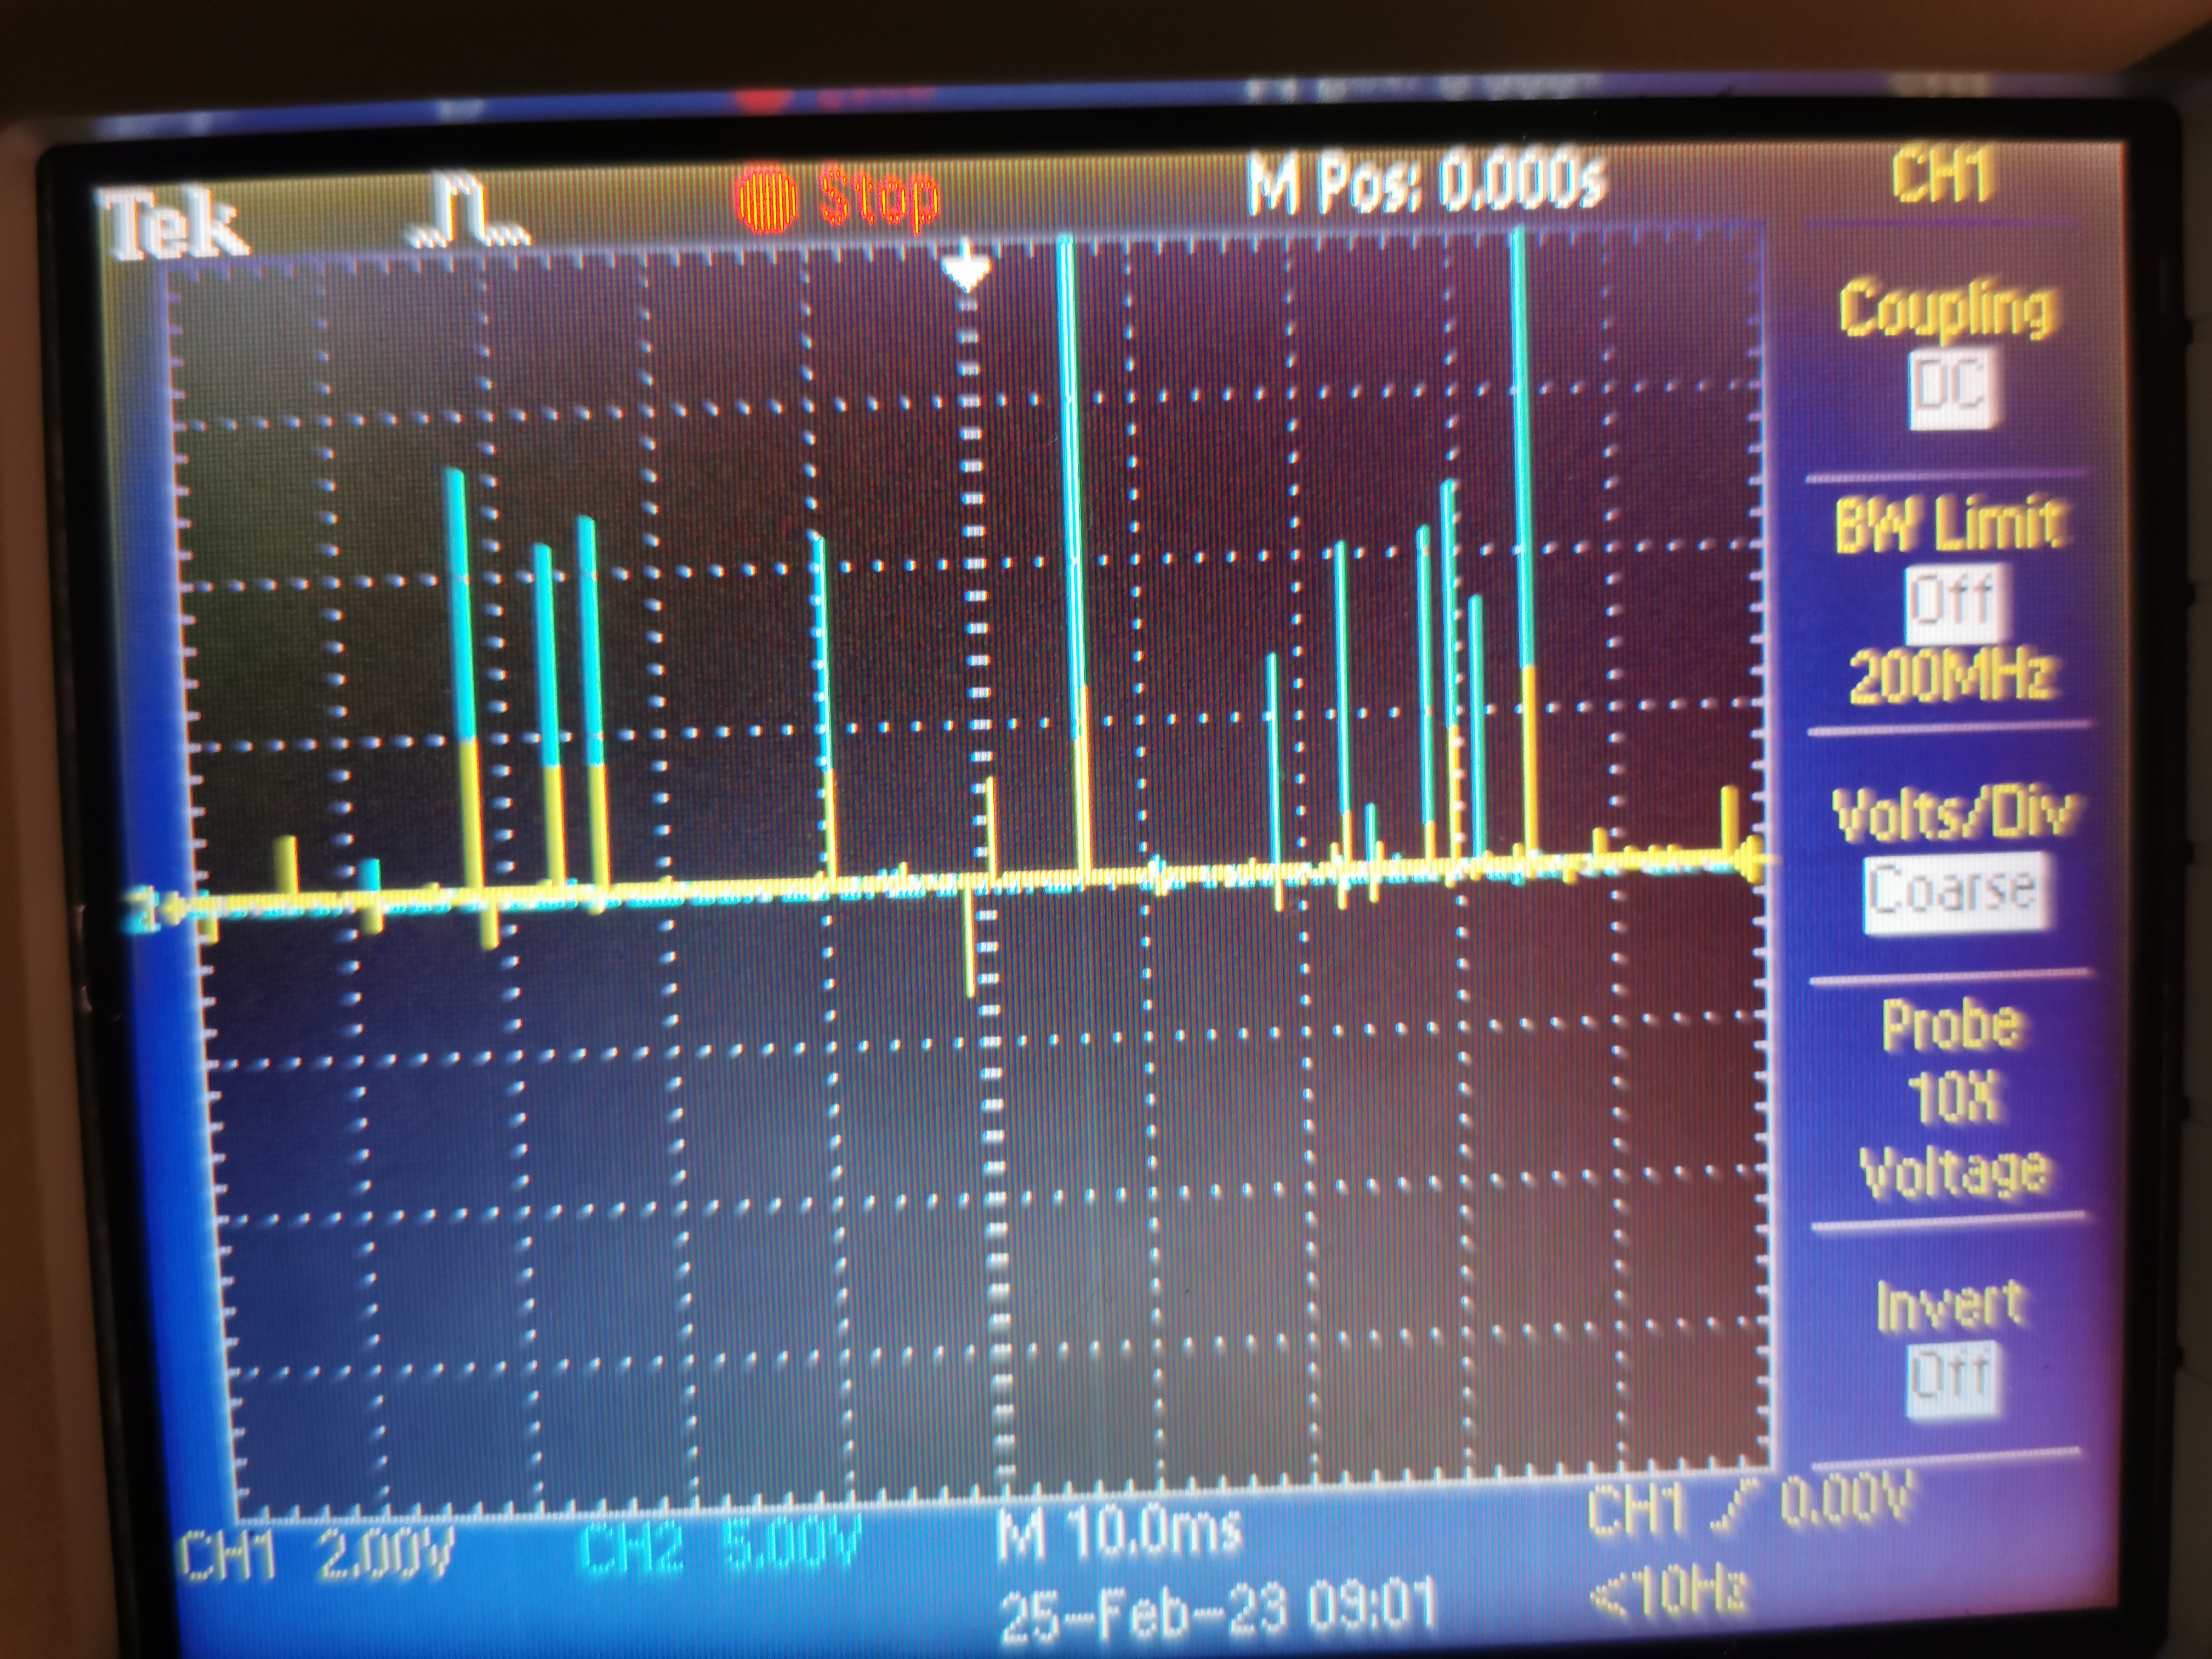
\includegraphics[width = 8cm]{BB_attenuate.jpg}
    \caption{Attenuation of SPCM AQ4C output signals to 3.3V logic.}
    \label{fig:signals}
\end{figure}

\subsection{Software}

The software used to drive the Altera-based CCM (ACCM) is taken from Mark Beck's
website. The advantage of the ACCM over the old CCM is that it can be modified for use
with a wide variety of other experiments, such as testing Bell's inequality, local realism, single
photon polarization states, and more. Some of the experiments require some additional upgrades
in equipment, but the core software can all be executed on the ACCM.

We validate the ACCM by performing a basic experiment with the maglite torch.
We hook the ACCM up with the coincidence counting library in labview. Through the front panel,
we observe that we are getting counts, and we also observe that we have count fluctuations that
are consistent with expectations when the torch is moved around. We take data for three different positions
of the maglite torch and observe some concerning results shown in table \ref{tab:fpga_res}.
\begin{table}[H]
    \centering
    \begin{tabular}{|l|l|}
    \hline
    \textbf{Trial Number} & \textbf{$\alpha$} \\ \hline
    1   & 36.43                  \\ \hline
    2        & 62.70                   \\ \hline
    3        & 42.10                   \\ \hline
    \end{tabular}
    \caption{Table of $\alpha$ values for different trials with the ACCM.}
\end{table}\label{tab:fpga_res}
These results are highly inconsistent with the outputs we expect for the torch source
and suggest an excessive coincidence count. There are further issues in the ACCM that need to be fixed.

\subsection{Possible Problems}

Some additional refinements and improvements can be made to the ACCM setup to possibly
resolve some of the problems that we have observed. One major improvement would be to
design the voltage divider circuit in a CAD program such as Altium and create a PCB.
The current circuit involves a somewhat unreliable and unrobust perfboard configuration that
likely will not hold up to student use in the future and can be slightly unreliable. Issues in the
breakout board can cause noisy extra counts or kill signal and is detrimental to the overall experiment.

An additional area that can be investigated further with the ACCM is the labview software provided
with the hardware. I have not been able to dig into the software too much, and have not found out a way
to run tests with varied coincidence windows or with some of the other bells and whistles provided
with the software. Perhaps the fine-tuning of certain settings could resolve the current issues
with $\alpha$ measurements.

\section{Extensions}

Aside from the possible fixes to the ACCM setup, another major extension to the single photon experiment
would be to try and utilize the full capabilities of the Altera board and implement some of the additional
labs on Mark Beck's page. This could lead to the development of a full lab course that covers much more
experiments in quantum mechanics and has a greater applied bend. The lab setups are all well-documented on Mark's
website and should be fairly straightforward to set up, though they will require some additional
equipment.

As for the random number generation component of this project, it would be interesting
for someone to take the random number generation capabilities of the current set-up and extend it
to a remote web-app that enables users to remotely run experiments and generate passwords.
This would likely involve the addition of some servos and controllers that allow a user to remotely
toggle on and off the experiment, as well as take the outputs of the labview program and directly
sending them into automated processing that directly turns the string of random numbers into a password that
is then streamed to the user.

Another set of fun extensions to the random number generation is to investigate how various
attack schemes can alter the experiment. For instance, if the room were to be heated by an attacker,
causing upwards laser drift and an increase in the Poissonian mean, then the output "random" bits
would be biased towards a certain direction. One could explore various methods of attacking this experiment
and also various methods of prevention, such as periodic re-calibration and validation of the set-up.
% -------------------------------------------------------------------------------------
% REFERENCES
% -------------------------------------------------------------------------------------
\bibliography{citations.bib}

% -------------------------------------------------------------------------------------
% END DOCUMENT
% -------------------------------------------------------------------------------------
\end{document}